\chapter{Tehtävä 3: 
\label{chap:Teht=0000E4v=0000E4-2}}

\section{yhdistä() -metodin palautuvat viittaukset}

\label{}

Muodostetaan ensin tehtävän tarvitsema oliohierarkia kirjoittamalla luokat
muotoon:

\begin{javacode}
class Eucarya {}
class Animalia extends Eucarya {}
class Chordata extends Animalia {}
ja niin edelleen
\end{javacode}

Tuloksena saadaan oliohierarkia (kuva \ref{Lajisto}). 

\begin{figure}
\centering 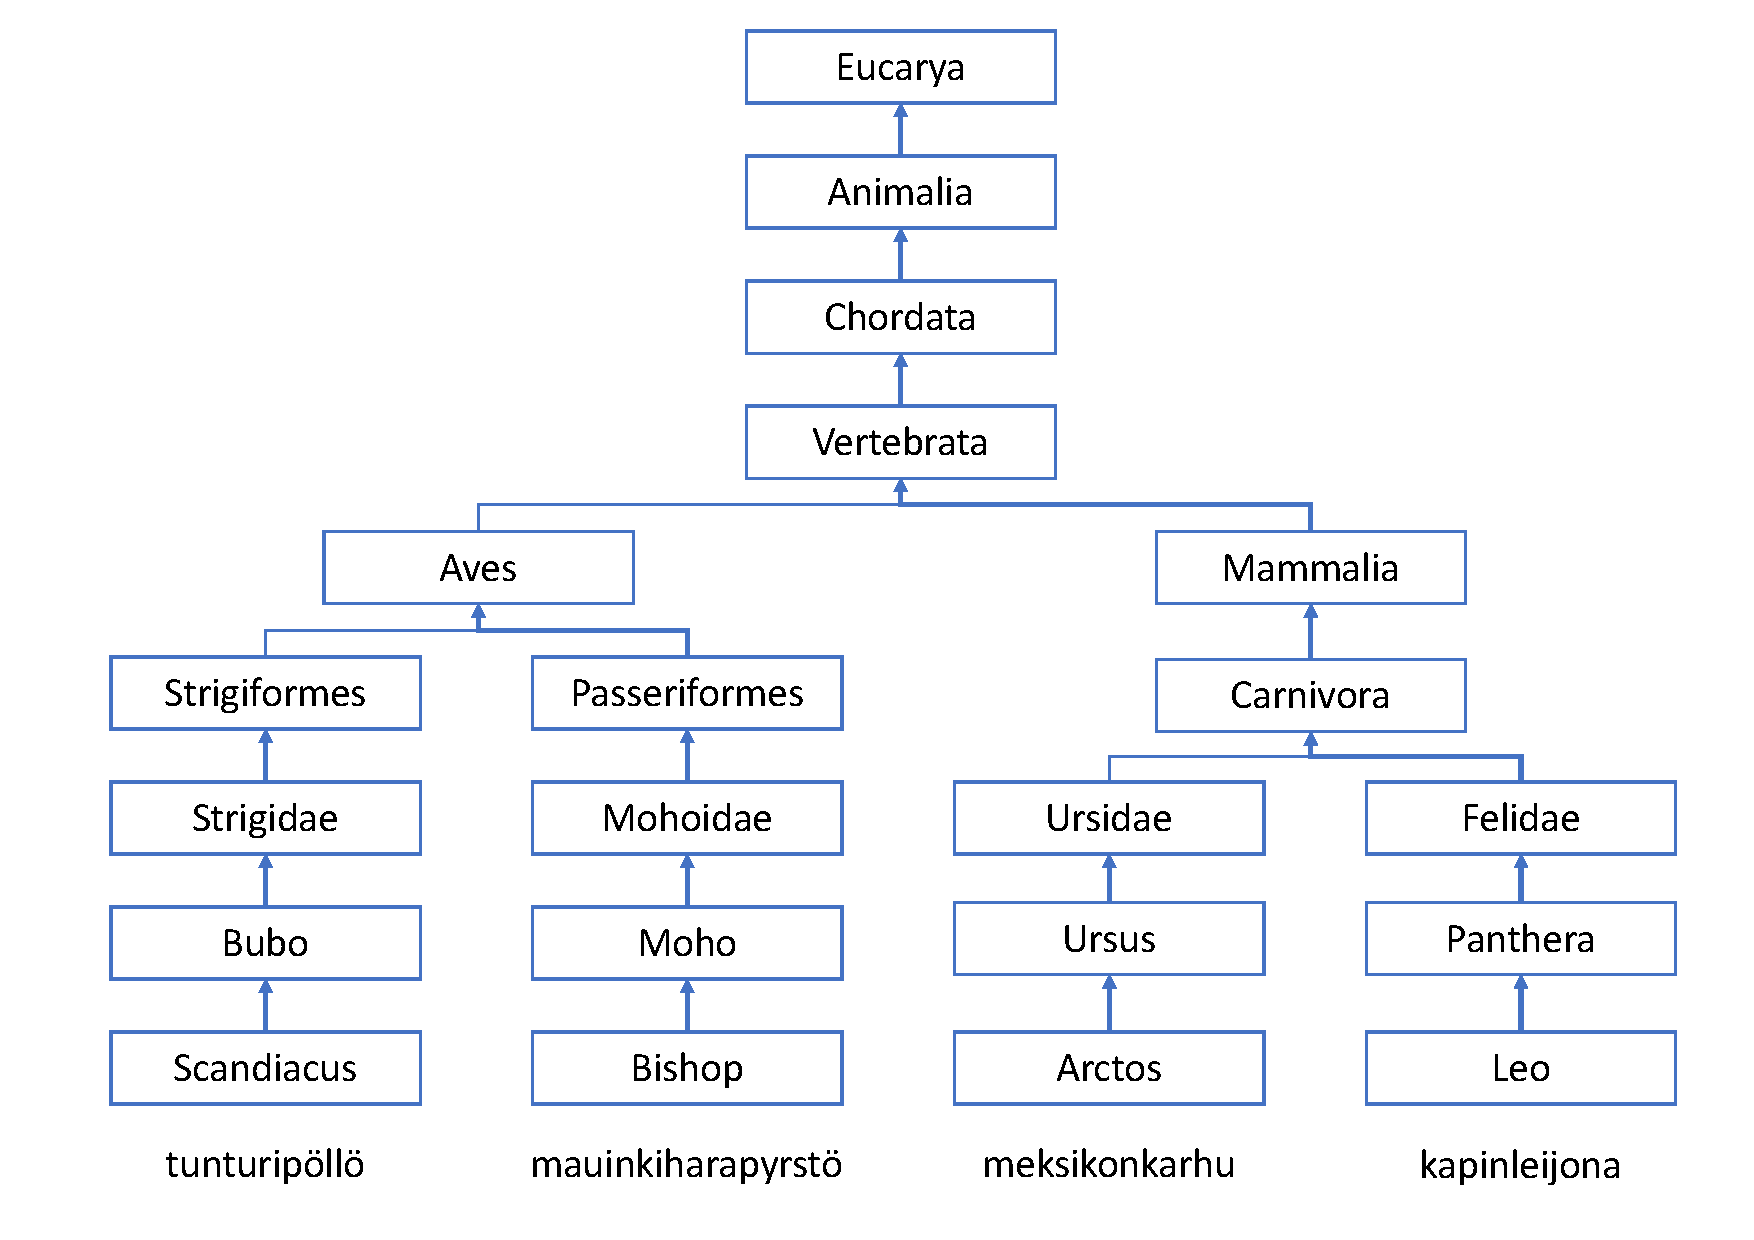
\includegraphics[width=0.5\textwidth]{kuvat/Lajisto}
\caption{Luokkakaavio lajiston periytyvyydestä}
\label{Lajisto} 
\end{figure}

Yhdistä() -metodi voidaan toteuttaa ylikuormitettuna käyttämällä apuna metodia
getLevel(), joka antaa olion lajitason kokonaislukuna niin, että Eucarya -luokan
oliot palauttavat luvun 0, Animalia 1:sen jne\ldots getLevel() ja yhdistä()
-metodit esitetään seuraavaksi koostetusti niin, että luokkahierarkia jätetään
esittämättä.

\begin{javacode}
/**
 * Level kuvaa kuinka korkealla eliö on lajistotasolla
 * @return 0 ellei eliö ole korkeampaa luokkaa
 */
public int getLevel() {
	return 0;
}

/**
 * Rekursiivinen määrittely korkeammille luokille
 */
@Override
public int getLevel() {
	return super.getLevel()+1;
}
	
/**
 * 
 * @param input Saman lajitason eliö
 * @return Taulukko muodossa {this,eliö}, jos eliö on samalla tasolla. 
 */
public Eucarya[] yhdistä(Eucarya eliö) {
	if (this.getLevel() == eliö.getLevel()) {
		return new Eucarya[] {this,eliö};
	}
	return new Eucarya[] {};
}

/**
 * 
 * @param eliöTaulukko
 * @return Taulukko, johon on lisätty this. Palauttaa tyhjän taulukon jos eliöt
 * eivät ole samalla tasolla.
 */
public Eucarya[] yhdistä(Eucarya... eliöTaulukko) {
	Eucarya[] result = new Eucarya[eliöTaulukko.length + 1];
	result[0] = this;
	
	for (int i = 0; i < eliöTaulukko.length; i++) {
		if (this.getLevel() != eliöTaulukko[i].getLevel()) {
			return new Eucarya[] {};
		}
		result[i+1] = eliöTaulukko[i];
	}
	return result;
}
\end{javacode}

Testausta varten käytetään tulosta() -metodia joka selittää lyhyesti eliöiden lajitason. 

\begin{javacode}
public static void tulosta(String otsikko, Eucarya... taulukko) {
	System.out.println(otsikko);
	for (int i = 0; i < taulukko.length; i++) {
		System.out.println("Eliön lajitaso " + i + ": " + taulukko[i].getClass());
	}
}
\end{javacode}

Jolloin voidaan suorittaa tehtävässä kysytty algoritmi:

\begin{javacode}
Eucarya[] taulukko = maunkiharapyrstö.yhdistä(meksikonkarhu);
tulosta("maunkiharapyrstön ja meksikonkarhun yhdistelmä",taulukko);

taulukko = kapinleijona.yhdistä(meksikonkarhu);
tulosta("kapinleijonan ja meksikonkarhun yhdistelmä",taulukko);

taulukko = kapinleijona.yhdistä(maunkiharapyrstö.yhdistä(meksikonkarhu));
tulosta("meksikonkarhun, maunkiharapyrstön ja kapinleijonan yhdistelmä",taulukko);

//maunkiharapyrstön ja meksikonkarhun yhdistelmä
//Eliön lajitaso 0: class Bishop
//Eliön lajitaso 1: class Arctos
//kapinleijonan ja meksikonkarhun yhdistelmä
//Eliön lajitaso 0: class Leo
//Eliön lajitaso 1: class Arctos
//meksikonkarhun, maunkiharapyrstön ja kapinleijonan yhdistelmä
//Eliön lajitaso 0: class Leo
//Eliön lajitaso 1: class Bishop
//Eliön lajitaso 2: class Arctos
\end{javacode}

Huomion arvoista on, että taulukkojen yhdistäminen tapahtuu niin, että jokainen
eliö tulee olla samalla lajitasolla. Jos ylläolevan koodin rivillä 7 tapahtuisi
tilanne, jossa sisempien sulkujen sisällä yhdistäminen ei onnistuisi, niin
tulostuisi pelkästään taulukko, jossa olisi kapinleijona. Olisi siis
turvallisempaa toteuttaa rivi 7 käyttäen yhdistä() -metodia seuraavalla tavalla:

\begin{javacode}
taulukko = kapinleijona.yhdistä(new Eucarya[] {maunkiharapyrstö,meksikonkarhu});
\end{javacode}

Jolloin taulukko olisi varmasti tyhjä, jos jokin eliöistä on mahdotonta yhdistää
kapinleijonan kanssa.

\section{Olio-taulukon varianssi}

\label{}

Jos ajetaan tehtävänohjeistuksen mukainen koodi:

\begin{javacode}
Olio[] oliot = new Olio[] { new Olio() };
oliot[0] = new Olio(); // OK
Object[] objektit = oliot;
objektit[0] = new Olio(); // OK 
objektit[0] = new Object();
System.out.println("Onnistui");
\end{javacode}

Jossa Olio -luokka on Object -luokan alaluokka, koska kaikki luokat, joilla on
olioesiintymiä ovat Object -luokan alaluokkia. Listan luomisen jälkeen luodaan
viittaus objektit oliot-taulukkoon. Viittaus ei kumminkaan pysty muuttamaan
taulukkoa ylemmän luokan taulukoksi vaan tämä tulisi konstruoida uudelleen.
Ohjelman ajo siis keskeytyy ajonaikaiseen virheeseen jossa objektit
viittauksella yritetään ylikirjoittaa Object -luokan olio taulukkoon, jossa voi
olla vain Olio -luokkaa tai tämän aliluokkia, jolloin luokkaviittauksen
invarianssi ei päde.

Koodi voidaan korjata toimivaksi kirjoittamalla rivi 3 seuraavalla tavalla:

\begin{javacode}
Object[] objektit = new Object[]{oliot[0]};
\end{javacode}

Jolloin objektit viittaa uuteen taulukkoon, jossa voi olla mitä tahansa olioita.

\section{Solmu -luokan periytymisongelmat}

\label{}

Ensimmäisenä ongelmana voisi olla solmujen väliset toimenpiteet. Voisi olla
epäselvää, että onko erikoistettujen solmujen equals -metodi sama, kuin Solmu-
luokan solmujen. Siinä tapauksessa equals -metodin palautus erikois- ja
normaalisolmun välillä riippuisi siitä kummalta kysytään. Tämä voi olla
ongelmallista, kun halutaan vertailla mitkä solmut ovat oikeasti samoja.

Jos yritetään mallintaa vaikka tiekarttaa jota kuvataan suunnattuna graafina,
niin solmujen erikoistaminen siinä tapauksessa, että kaupungin läpi ajaminen
vaihtelisi riippuen siitä löytyykö kehätietä vai tuleeko autoilijan ajaa
keskustaan. Tätä voitaisiin kuvata solmun ominaisuutena, mutta silloin tulisi
kirjoittaa paljon suunnattuja graafeja uudelleen, koska matkan laskemiseen
käytettävä algoritmi tulisi toimia eri tavalla.

Voitaisiinkin miettiä voisiko kaupunkien läpi ajaessa parempi kuvata kaarilla ja
merkata niihin, että matka on pidempi. Se tarkoittaisi sitä, että jokainen kaari
joka on vaikka yhteydessä Varkauteen tulisi painottaa suuremmaksi. Nyt matkan
laskemisalgoritmia ei tarvitsisi kirjoittaa uudestaan.

\section{Periytymisratkaisujen arvioimista}

\label{}

\subsection{PeliObjekti matopelissä}

Jos haluttaisiin tehdä PeliObjekti, jossa olisi yhtenäisenä piirteenä ainoastaan
se, että niillä kaikilla olisi olemassa jotkin koordinaatit, jotka kertovat
missä kohtaa pelialueella ne ovat. Tämä olisi huono ratkaisu, koska
erikoistumista ei tapahdu tarpeeksi ja eteen tulisi peliä laajentaessa jossain
vaiheessa invarianssiongelmia.

Olisi järkevämpää tehdä rajapinta ``koordinaatillinen'', jolla merkattaisiin kaikki
luokat joilla olisi koordinaatit. Rajapintaan voisi tehdä säännön, että jokainen
tämän rajapinnan luokka toteuttaa erilaiset koordinaatteihin liittyvät metodit.
Jos PeliObjekti vaikka koostuisi useasta osasta, niin annaKoordinaatit() -metodi
voisi palauttaa esimerkiksi näiden usean osan koordinaattien vektori-keskiarvon.
Näin useasta osasta koostuva peliobjekti voisi säilyttää oman abstraktionsa
useampiosaisena systeeminä.

\subsection{Banaani-luokka toteuttaa rajapinnan Painovoima}

Jos Banaani-luokka toteuttaa rajapinnan painovoima, niin voidaan kohdata
ongelmia pelimoottorin kanssa. Fysiikan lakien mukaan painovoima, on enemmänkin
massallisten kappaleiden väliseen vuorovaikutukseen liittyvä ominaisuus. Tämä
ratkaisu rajaa pelimekaniikan tilanteeseen, jossa painovoima voi tapahtua vain
alaspäin. Lisäksi Painovoima rajapinta tekisi pelimoottorin kannalta hyvin vähän
asioita: lähinnä määräisi, että tähään olioon vaikuttaisi alaspäin suuntautuva
kiihtyvyys.

Koska kaikki kappaleet luonnossa kiihtyvät yhtä nopeasti alaspäin, niin
mielekkäämpää olisi vain tehdä luokka Kappale, johon olisi sisäänkirjoitettuna
painovoiman aiheuttama kiihtyvyys vektorina.

\subsection{Ympyrä perii ellipsin}

Ympyrä on ellipsin erikoistapaus, jossa säteen suuruus pysyy vakiona. Jos
halutaan mallintaa ympyrää matemaattisesti, niin tämä voi olla hyvä idea.
Toisaalta näin tehdessä laskennallinen rutiini hidastuu, koska jokaisen ympyrän
kuvaaminen ellipsinä on hitaampaa, kuin että tehtäisiin oma Ympyrä-luokka.
Omassa Ympyrä -luokassa voitaisiin laskentaa nopeuttaa ja erikoistaa.

\subsection{Ellipsi perii ympyrän}

Ellipsin periessä ympyrän erikoistaminen tapahtuu toisin. Tässä tilanteessa
ympyrän käsitettä yleistetään lisäämällä siihen ominaisuuksia niin, että
ellipsille ominaiset piirteet voidaan mallintaa. Tämä on hyvä idea, koska
ellipsillä on paljon ominaisuuksia, jotka ovat samankaltaisia ympyrän kanssa:
esim. keskeissäde ja keskipiste.

\subsection{Neperin luku peritään luokasta Number}

Luonnon vakioiden tai matemaattisten tunnuslukujen tallentaminen kannattaa tehdä
joko omaksi singulaariseksi olioksi tai Number -luokan staattiseksi
ominaisuudeksi. Neper -olioita ei tarvita laskutoimituksissa useita kappaleita,
joten tällainen periminen on aivan turhaa.

\subsection{Stack perii Vector -luokan}

Stack -luokalla halutaan lisätä Vector -luokkaan ominaisuus poistaa viimeinen
jäsen tai lisätä uusi jäsen ensimmäiseksi listassa. Vector -luokassa jäseniä
poistetaan tietyistä indekseistä ja uusi jäsen lisätään aina viimeiseksi. Koska
Stack -luokassa halutaan käyttää Vector luokan toiminnallisuutta periminen on
perusteltua. 

Stack -luokka voisi periä myös jonkin muun List -luokan, jolloin pystyttäisiin
muodostamaan sama toiminnallisuus. Tähän voitaisiin päätyä, jos Stack -luokan
käytännöt eivät muistuttaisi niin paljon Vector -luokkaa.
